%% LyX 1.6.7 created this file.  For more info, see http://www.lyx.org/.
%% Do not edit unless you really know what you are doing.
\documentclass[12pt,a4paper,ngerman,english,intoc,bibtotoc,idxtotoc,BCOR10mm,titlepage,tablecaptionabove,oneside]{scrbook}
\usepackage{lmodern}
\renewcommand{\sfdefault}{lmss}
\renewcommand{\ttdefault}{lmtt}
\usepackage[T1]{fontenc}
\usepackage[latin9]{inputenc}
\usepackage{fancyhdr}
\pagestyle{fancy}
\setcounter{secnumdepth}{3}
\setlength{\parskip}{\medskipamount}
\setlength{\parindent}{0pt}
\usepackage{babel}

\usepackage[authoryear]{natbib}

\def\CC{{C\nolinebreak[4]\hspace{-.05em}\raisebox{.4ex}{\tiny\bf ++}}}

\usepackage{datetime}
\renewcommand{\dateseparator}{.}

\usepackage{amsmath}
\usepackage{graphicx}
\usepackage{amssymb}
\usepackage{nomencl}
% the following is useful when we have the old nomencl.sty package
\providecommand{\printnomenclature}{\printglossary}
\providecommand{\makenomenclature}{\makeglossary}
\makenomenclature
\usepackage[unicode=true, 
 bookmarks=true,bookmarksnumbered=true,bookmarksopen=true,bookmarksopenlevel=1,
 breaklinks=false,pdfborder={0 0 0},backref=false,colorlinks=true,citecolor=blue,linkcolor=magenta]
 {hyperref}
\hypersetup{pdftitle={Your Title},
 pdfauthor={Jie Bao},
 pdfsubject={Dissertation zur Erlangung des Doktorgrades der Fakult�t f\"ur Biologie der Albert-Ludwigs-Universit�t Freiburg im Breisgau},
 pdfkeywords={Ph.D. thesis},
 pdfpagelayout=OneColumn, pdfnewwindow=true, pdfstartview=XYZ, plainpages=false}

\makeatletter

%%%%%%%%%%%%%%%%%%%%%%%%%%%%%% LyX specific LaTeX commands.
\pdfpageheight\paperheight
\pdfpagewidth\paperwidth

\DeclareRobustCommand*{\lyxarrow}{%
\@ifstar
{\leavevmode\,$\triangleleft$\,\allowbreak}
{\leavevmode\,$\triangleright$\,\allowbreak}}

%%%%%%%%%%%%%%%%%%%%%%%%%%%%%% User specified LaTeX commands.
% print no date
\date{}

% increase link area for cross-references and autoname them
\AtBeginDocument{\renewcommand{\ref}[1]{\mbox{\autoref{#1}}}}
\newlength{\abc}
\settowidth{\abc}{\space}
\addto\extrasenglish{
 \renewcommand{\equationautorefname}{Eq.\hspace{-\abc}}
 \renewcommand{\sectionautorefname}{Sec.\negthinspace}
 \renewcommand{\subsectionautorefname}{Sec.\negthinspace}
 \renewcommand{\subsubsectionautorefname}{Sec.\negthinspace}
 \renewcommand{\figureautorefname}{Fig.\negthinspace}
 \renewcommand{\tableautorefname}{Tab.\negthinspace}
}

% in case somebody want to have the label "equation"
%\renewcommand{\eqref}[1]{equation~(\negthinspace\autoref{#1})}

% that links to image floats jumps to the beginning
% of the float and not to its caption
\usepackage[figure]{hypcap}

% the pages of the TOC is numbered roman
% and a pdf-bookmark for the TOC is added
\let\myTOC\tableofcontents
\renewcommand\tableofcontents{%
  \frontmatter
  \pdfbookmark[1]{\contentsname}{}
  \myTOC
  \mainmatter }

% make caption labels bold
\setkomafont{captionlabel}{\bfseries}
\setcapindent{1em}

% enable calculations
\usepackage{calc}

% fancy page header/footer settings
\renewcommand{\chaptermark}[1]{\markboth{#1}{#1}}
\renewcommand{\sectionmark}[1]{\markright{\thesection\ #1}}
%\lhead[\fancyplain{}{}]{\fancyplain{}{\rightmark}}
\rhead[\fancyplain{}{\leftmark}]{\fancyplain{}{}}
\lfoot[\thepage]{}
\rfoot[]{\thepage}
\cfoot{}

% increase the bottom float placement fraction
\renewcommand{\bottomfraction}{0.5}

% avoid that floats are placed above its sections
\let\mySection\section\renewcommand{\section}{\suppressfloats[t]\mySection}

% widen the space for the nomenclature entry labels
\renewcommand{\nomlabelwidth}{2.5cm}

\makeatother

\begin{document}
\selectlanguage{ngerman}%

\subject{Dissertation zur Erlangung des Doktorgrades der 
Fakult�t f\"ur Biologie
der Albert-Ludwigs-Universit�t Freiburg im Breisgau}

\selectlanguage{english}%

\title{A Network View of the Dynamic Transcriptome Response}


\author{Jie Bao}


\date{}

\selectlanguage{ngerman}%

\publishers{
\includegraphics[width=0.4\columnwidth]{fig/Uni_Logo-Grundversion_E1_A4_CMYK}\vspace{\baselineskip}\\
Albert-Ludwigs-Universit�t Freiburg im Breisgau\\
Fakult�t f\"ur Biologie\\
%Institut f�r zzz\vspace{-3cm}
}


\lowertitleback{\textbf{Dekan}\smallskip{}
\\
Prof. Dr. Ad Aertsen\bigskip{}
\\
\textbf{Promotionsvorsitzender}\smallskip{}
\\
Prof. Dr. Samuel Rossel\bigskip{}
\\
\textbf{Betreuer der Arbeit}\smallskip{}
\\
Dr. Hauke Busch\bigskip{}
\\
\textbf{Datum der Promotion (only necessary for final publication)}\smallskip{}
\\
xx.yy.zzzz}

\selectlanguage{english}%

\maketitle

\thispagestyle{empty}
\setcounter{page}{0}
\vspace*{\fill}
\begin{quote}
The whole is more than the sum of its parts. 
\begin{flushright}
--- Aristotle\\
\end{flushright}
\end{quote}
\vskip 1in
\begin{quote}
Theorie ohne Praxis ist 
wirkungslos, Praxis ohne Theorie ist blind.
\begin{flushright}
--- Immanuel Kant\\
\end{flushright}
\end{quote}
\vfill
\noindent

\cleardoublepage{}

\lhead[\fancyplain{}{}]{\fancyplain{}{\rightmark}}

\tableofcontents{}
\listoffigures

\cleardoublepage{}

\pagestyle{plain}

\begin{itemize}
  \item introduction
  \begin{itemize}
    \item signal flow: protein interaction network $\rightarrow$ transcriptome
    \item failure of biomarker
    \item complexity can only be understood within the
      network context~\citep{Barabasi2012}, Understanding a complex network's 
      structure is beneficial to understanding its function
  \end{itemize}
  \item network dynamics and topology
  \begin{itemize}
    \item fireworks: sequence of events, dynamics
    \item elephant in the room: what we can and cannot see from
    the transcriptome data
    \item gene expression heavy-tailed distributed, discuss 
    bimodal distribution 
    \item normalization assumption: most genes do not change
    expressions
    \item few genes respond: sparsity assumption in reverse-%
    engineering
    \item Network inference in the yeast is already hard because absence of correlation
    between TF expression and activity~\cite{Marbach2012}
    \item CRNT: structure of the reaction network determines the number and type of
    steady states
  \end{itemize}
  \item signal flow
  \begin{itemize}
    \item TF important in disease, but not detectable: many of the TFs that regulate physiological
    targets are constitutively present, and their activity is determined
    by posttranslational modifications such as phosphorylation%
    ~\cite{Messina2004}
  \end{itemize}
  \item conclusions
\end{itemize}

%\include{Summary}
%
%\include{Zusammenfassung}
%
%\cleardoublepage{}
%
%\pagestyle{fancy}\lhead[\fancyplain{}{\chaptername\;\thechapter}]{\fancyplain{}{\rightmark}}
%
%\include{chapter-1}

% $Id: network.tex 2 2012-09-13 23:13:00Z jbao $
\chapter{Network dynamics and topology}

Cells initiate and control decisions like migration, proliferation or differentiation through the intricate, yet
coordinated, regulation of large gene interaction networks. 
As a consequence, there is  well orchestrated time-sequential regulation of protein pathways, resulting in and regulated by a  global change in gene expression.
Gaining insight into the necessary and suffient regulators controlling cellular decisions  is therefore difficult. 
The central questions are, how to bridge the large data set to regulator or key players, how does the cell come to unique and well defined decisions despite the underlying complexity?

Systems theory points to ways how complex systems are regulated and obey common rules with respect to their organisation and dynamic responses~\citep{Kauffman1993}. 
In order to tackle the complexity of such systems, 
one usually works with
an abstract
representation or a graph consisting of different molecules as nodes and the 
interactions among them as edges. In order to understand the
behavior of complex systems, one has to understand both
the topological and dynamical properties of networks. In this chapter, we first
introduce some graph theoretical concepts, we then investigate the dynamics and
topology in \emph{in silico} networks, finally we present a biological application.

\section{Complex networks in biology and beyond}
Biological phenomena are described in the context of a network
at all spatial and temporal scales, from food web~\citep{Williams2000}, 
neuronal network~\citep{White1986}, gene regulatory networks~%
\citep{Kauffman1969,Gama-Castro2008,Abdulrehman2011},
protein-protein interaction networks~\citep{Jeong2001,Stelzl2005}
to metabolic network~\citep{Herrgaard2008}.

The study of networks dates back to the K\"onigsberg
problem from Leonhard Euler in the 18th century. The initial
problem deals with seven bridges across the river in the city
of K\"onigsberg, and the aim is to find a walk through the 
city that would cross each bridge once and only once, to which
Euler proved that there is no solution. For a long time,
graph theory remains a specialized and abstract mathematical 
discipline. Not until the publication of the first 
small-world network model~\citep{Watts1998} did people
realize that there is a class of networks, which is neither
purely random nor purely regular and can represent most of
the real-world structures, ranging from Internet, power grid
to collaboration graph of film actors, and also biological
networks.

Study of biological networks has been largely inspired by the theoretical 
analyses of other types of networks~\citep{Barabasi2004}. In recent years, 
there is also increasing interest in the comparison between biological and
other networks. For instance, the transcriptional regulatory network of 
\emph{E. coli} is found to have a triangle-like hierarchical 
structure, whereas the Linux kernel displays rather an inverse-triangle
hierarchy, which again is due to different design principles of the two 
systems: robustness for biological systems and cost effectiveness for 
software systems~\citep{Yan2010}.
Such findings highlight the hypothesis of \emph{form follows function}, or 
the function of complex networks can be attributed to their distinct structural 
properties.

\section{Network topology}
There are a variety of measures that characterize the topology of networks,
some capture local network topology, yet others are global topology measures.

\subsection{Topological measures}

\subsubsection{Degree and degree distribution}
The \emph{degree} (or connectivity) $k_i$ of a node $i$ is the number of edges 
connecting the node, in case of directed networks, one further distinguishes
between incoming ($k_i^{in}$) and outgoing degree ($k_i^{out}$). Then the total 
degree is defined as $k_i = k_i^{out} + k_i^{in}$. A list of the node degrees 
of a network is called the \emph{degree sequence}.

The \emph{degree distribution} $P(k)$, or the fraction of nodes in the graph 
$G$ having degree $k$, is probably the most basic topological 
characterization of a graph. It has been shown that the degree distribution of
a neuronal network determines its global oscillatory state~\citep{Roxin2011}, 
and the number of driver nodes in a network is determined mainly by the 
network's degree distribution, assuming linear dynamics at
individual nodes~\citep{Liu2011}.

\subsubsection{Shortest path and betweenness}
\emph{Shortest paths} $d_{ij}$ from node $i$ to node $j$ play an important 
role in the transport and communication 
within a network. Although highly efficient algorithm exists to perform
route planning such as in Google Maps~\citep{Sanders2005}, common algorithms
for calculating shortest paths are Dijkstra's algorithm for weighted networks
and the breadth-first search for unweighted networks.

An extension of the shortest path is a measure of the importance of a given 
node defined by the sum of the fraction of all-pairs shortest paths that pass 
through it, or the 
\emph{betweenness} $b_i$ of a node $i$ is given by
\begin{equation}
b_i = \sum_{s,t \in N} \frac{\sigma(s,t|i)}{\sigma(s,t)},
\end{equation}
where $N$ is the set of nodes, $\sigma(s,t)$ is the number of shortest paths 
between node $s$ and $t$, and $\sigma(s,t|i)$ is the number of those paths 
passing through the node $i$ other than $s$ and $t$.

\subsubsection{Motif}
A \emph{network motif} $M$ is a pattern of interconnections occurring in complex 
networks at a number that is significantly higher than those in randomized 
networks~\citep{Milo2002,Shen-Orr2002}. The statistical significance of M is 
then described by the $Z$-score, defined as
\begin{equation}
Z_M = \frac{n_M - \langle n_M^{rand} \rangle}{\sigma_{n_M^{rand}}},
\end{equation}
where $n_M$ is the number of times the subgraph $M$ appears in $G$, and 
$\langle n_M^{rand} \rangle$ and $\sigma_{n_M^{rand}}$ are, respectively, 
the mean and 
standard deviation of the number of appearances in the randomized network ensemble.
Motifs have been strongly linked to the information processing in networks, 
for example, the incoherent feedforward loop was shown to be able to detect
fold change in the input signal~\citep{Goentoro2009}.

\subsubsection{Community}
A \emph{network community} or module is a subnetwork with many edges joining
nodes of the same cluster and comparatively few edges joining nodes of 
different clusters. Since such communities can be considered as fairly 
independent compartments of a graph, they are usually also assigned 
a similar function, e. g., individual tissues or organs in the human body,
pathways within the cellular signal transduction network, a group of people
with common interest within the social network~%
\citep{Fortunato2010,Newman2012}.

There are now a zoo of algorithms to detect network communities, probably one
of the most influential methods is the algorithm proposed by \cite{Girvan2002},
which aims at the identification of edges lying between communities and their 
successive removal, a procedure that after some iterations
leads to the isolation of the communities. Most recently, \cite{Ahn2010b} 
suggested that each node in a network can in principle belong to more than 
one functional group, they therefore reinvented the definition of communities 
as groups of links rather than nodes and demonstrated this approach can uncover
natural overlap while revealing hierarchical organization of the network.

\subsection{Scale-free networks}
Together with the small-world network model, the scale-free network model~%
\citep{Barabasi1999} has
also attracted much attention in the research community. The basic idea of 
how a scale-free network and its power-law degree distribution comes into
existence is called preferential attachment. In other words, at each time
step of a growing network, a new node is added to a certain node in the 
network based on the probability that is proportional to the degree of the
given node, i.e. strongly connected nodes will get more and more connections,
popular nodes will be even more attractive. Such a model is able to reproduce
the power-law degree distribution observed in scale-free networks.

However, recent years have seen a critical assessment of the original 
scale-free model. On the one hand, several rigorous statistical analyses~%
\citep{Clauset2009,Khanin2006a} have shown that methods used to fit power-laws, such as 
least-squares, can produce substantially inaccurate estimates of the 
parameters. The authors concluded that in general the cumulative distribution
function is more robust than the probability distribution function against 
fluctuations due to finite sample sizes, especially in the tail of the 
distribution. It is also extremely difficult to distinguish between
the log-normal and power-law distribution. These results cast doubt on the
validity of most empirical characterization of power-law degree distribution
and the significance of classifying scale-free networks according to such
degree distributions.

On the other hand, there is now increasing evidence that mechanisms other than
preferential attachment can also lead to the empirical power-law degree 
distribution~\citep{Caldarelli2002}. For instance, a model of unspecific 
binding between proteins results exactly in a scale-free protein-protein 
interaction network~\citep{Deeds2006}.

\section{Network dynamics}
Here the network dynamics refers specifically to the dynamic response of the 
gene regulatory network. Such data are usually obtained from the microarray
time series. Microarray technology takes advantage of hybridization properties 
of nucleic acids and uses complementary molecules (probes) attached to a solid 
surface 
(chip) to measure the quantity of specific nucleic acid transcripts of 
interest that are present in a sample. A specialized scanner is used to 
measure the amount of hybridized target at each probe, which is reported as an 
intensity~\citep{Gentleman2005}. This intensity value is then interpreted as a
proxy for the level of gene expression. In order to characterize the global 
gene expression given a certain stimulus over time, one can perform the 
hybridization at multiple time points. The ultimate gene expression data are
thus multidimensional time series. Below we provide some of the methods that
can be used to analyse such data.

\subsection{Dimensionality reduction}
Dimensionality reduction is the transformation of high-dimensional data into 
a meaningful representation of reduced dimensionality~\citep{Maaten2009}, 
which is easy to both visualize and interpret. There are a variety of linear
and nonlinear dimensionality reduction algorithms 
(\ref{fig:dimension_reduction}). In this work, we heavily 
focus on the Euclidean distance based multidimensional 
scaling, which is equivalent to principal component analysis%
~\citep{Haerdle2003},
but more intuitive.

\begin{figure}[!ht]
\begin{center}
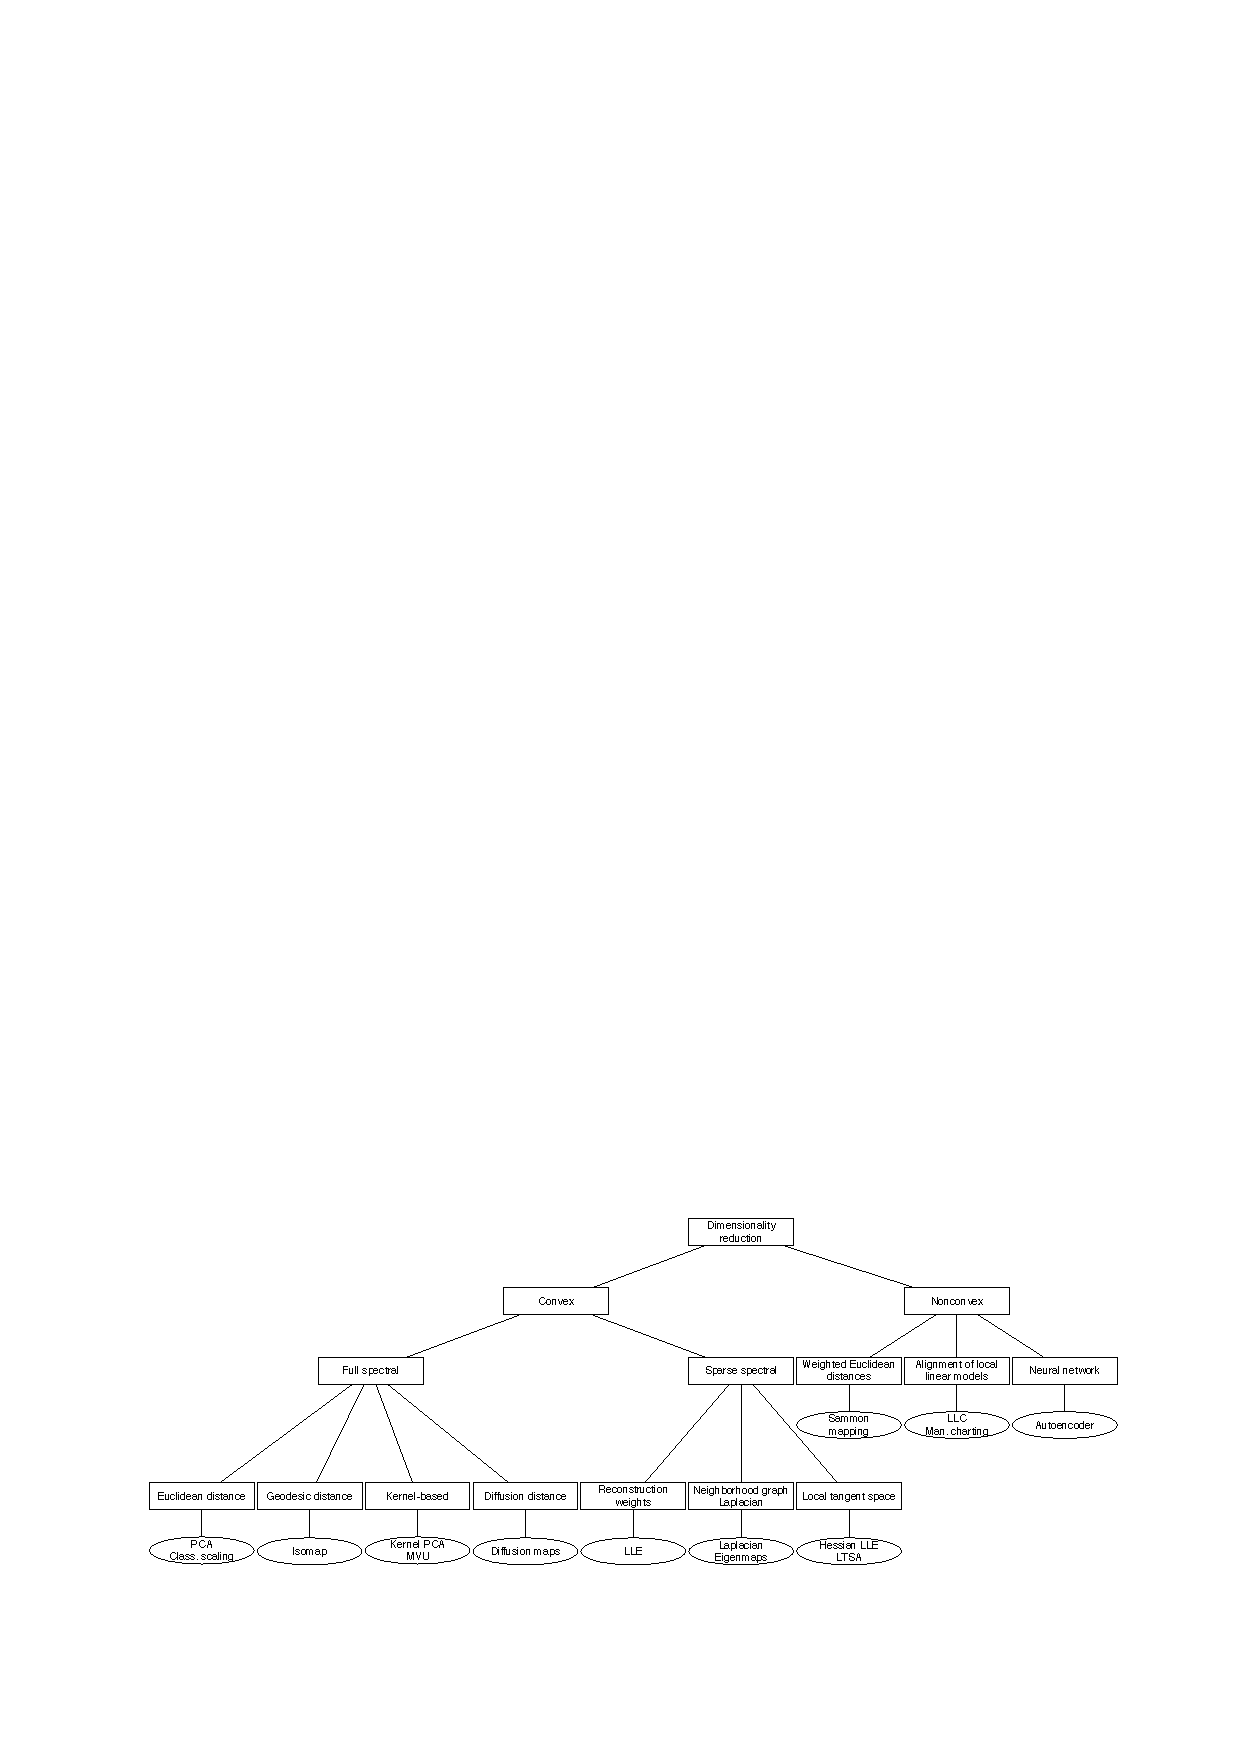
\includegraphics[width=\textwidth]{network/fig/dimension_reduction.pdf}
\end{center}
\caption[Dimensionality reduction algorithms]{
{\bf The taxonomy of dimensionality reduction algorithms.}
A non-exhaustive overview of diverse dimensionality reduction
techniques, taken from \cite{Maaten2009}.
}
\label{fig:dimension_reduction}
\end{figure}

\subsubsection{Multidimensional scaling}
Multidimensional scaling (MDS) is a family of algorithms that produces a spatial
representation of the dissimilarities between a number of entities $x_l^i \in 
\boldsymbol{X}_{n \times q}$ in $q$-dimensional space. In 
principle, MDS takes as input a symmetric $n \times n$ matrix 
\begin{equation}
  \boldsymbol{D} = \sqrt{\sum_{l=1}^q (x_l^i - x_l^j)^2}_{\substack{i \neq j,\\
    i,j=1...n}},
\end{equation}
which
describes the dissimilarities between the high-dimensional
entities. Those entities
are then represented by points in a low-dimensional space $\hat{x}_l^i \in 
\hat{\boldsymbol{X}}_{n \times d}$ ($d$ usually equals $2$ or
$3$ for ease of visualization), which are positioned
such that the pairwise distances between them 
\begin{equation}
  \hat{\boldsymbol{D}} = \sqrt{\sum_{l=1}^d (\hat{x}_l^i - \hat{x}_l^j)^2}_{\substack{
    i \neq j,\\i,j=1...n}}
\end{equation}
reflect as closely as possible  
the original
dissimilarities between the entities. 
The optimization of the spatial configuration is realized by the 
minimization of different stress functions.
We applied
here the HiT-MDS-2 algorithm (\citealp{Strickert2009}), where the
Pearson correlation of the original and the reconstructed distances 

\begin{equation}
  r(\boldsymbol{D}, \hat{\boldsymbol{D}}) = \frac{\sum_{i \neq j}^n (d_{ij} - \mu_{\boldsymbol{D}}
    ) \cdot (\hat{d}_{ij} - 
    \mu_{\hat{\boldsymbol{D}}})}{\sqrt{\sum_{i \neq j}^n (d_{ij} - \mu_{\boldsymbol{D}})^2} 
    \cdot \sqrt{
    \sum_{i \neq j}^n (\hat{d}_{ij} - \mu_{\hat{\boldsymbol{D}}})^2}}
\end{equation}
is maximized using a gradient descent approach.
Perticularly, $\boldsymbol{D} = (d_{ij})_{i,j=1...n}$ is Euclidean distance matrix of the
gene expression time series, and $\hat{\boldsymbol{D}} = (\hat{d}_{ij})_{i,j=1...n}$ 
is the 
Euclidean distance matrix of the reconstructed low-dimensional points. 
$\mu_{\boldsymbol{D}}$ and $\mu_{\hat{\boldsymbol{D}}}$ are the mean of matrix $\boldsymbol{D}$
and $\hat{\boldsymbol{D}}$ respectively.
\begin{eqnarray}
  \mu_{\boldsymbol{D}} = \frac{2}{n (n-1)} \sum_{i<j}^N d_{ij},\\
  \mu_{\hat{\boldsymbol{D}}} = \frac{2}{n (n-1)} \sum_{i<j}^N \hat{d}_{ij}.
\end{eqnarray}
%A stress function 
%\begin{equation}
%  s = -r(\boldsymbol{D}, \hat{\boldsymbol{D}})
%\end{equation}
%is minimized by gradient descent.
Throughout this work, the number of optimization cycles is fixed to be $100$.
The final configuration is centered, normalized by the largest dimension variance,
and rotated by Principal Component Analysis.

\subsubsection{Response strength metric}
\label{sec:response_strength}
In order to quantify the response strength of a single gene, we make use of 
MDS, namely by fitting a skewed Gaussian distribution (\citealp{Azzalini2003}) 
to the 2-D projection
of gene expression time series and assigning a $p$-value to each
gene according to its probability of being drawn from the fitted distribution.
We further take the negative logarithmic of the $p$-values as the response
strength metric. In so doing, a gene located at the periphery of the MDS
projection has a small $p$-value and thus a large response strength, whereas
central genes have small response strengths.

A multivariate skewed Gaussian distribution is defined as follows, suppose
$X$ is a $d$-dimensional random variable with a probability density function
\begin{equation}
f(X) = 2 \phi_d (X;\Omega) \ \Phi(\alpha^{\mathrm{T}} X), \quad X \in \mathbb{R}^d,
\label{eq:sn}
\end{equation}
where $\phi_d(X;\Omega)$ is the $N_d(0,\Omega)$ normal density function at $X$
with the correlation matrix $\Omega$, $\Phi(\alpha^{\mathrm{T}} X)$ is the 
cumulative distribution function of $N(0,1)$ evaluated at $\alpha^{\mathrm{T}} X$.
$\alpha$ is the shape parameter since when $\alpha=0$, Eq.~\ref{eq:sn} becomes
the regular normal probability density function again. $X$ can be further
linear transformed to
\[
Y = \xi + \omega X
\]
to include the location and scale parameter, $\xi$ and $\omega$ respectively.

Fitting of the skewed Gaussian distribution is performed with
the maximum likelihood method as implemented in the 
\texttt{R}
library \texttt{sn}, version 0.4-16.

\subsection{Modelling time series}
Another method to determine the dynamic response of a certain
gene is based on the work of \cite{Mar2009}. The difficulty 
in analyzing microarray time series data comes from the lack
of replicates in general at each time point. In order to 
circumvent this problem and increase the statistical power,
we take into account all data points in a time series at the
same time.

More specifically, we fitted cubic regression models to each 
individual gene expression profile. A cubic model was chosen 
because of the moderately large number of time points 
available to fit a model with four to eight parameters. 
For a single gene, both a full model and a reduced model are 
fitted to its time-course expression profiles under the 
stimulation and control condition. The full model specifies 
a set of parameters that capture the time-dependent curvature
of a gene's expression profile for each separate condition. 
In this way, the full model assumes that the expression 
profile is different across the two conditions, or

\subsection{Heave-tail response distribution}
Based on both the multidimensional scaling and full/reduced
model approach, we observe an invariant response pattern that only few genes are strongly induced upon stimulation, while the majority reacts
moderately (\ref{fig:response_strength}). 

\begin{figure}[!ht]
\begin{center}
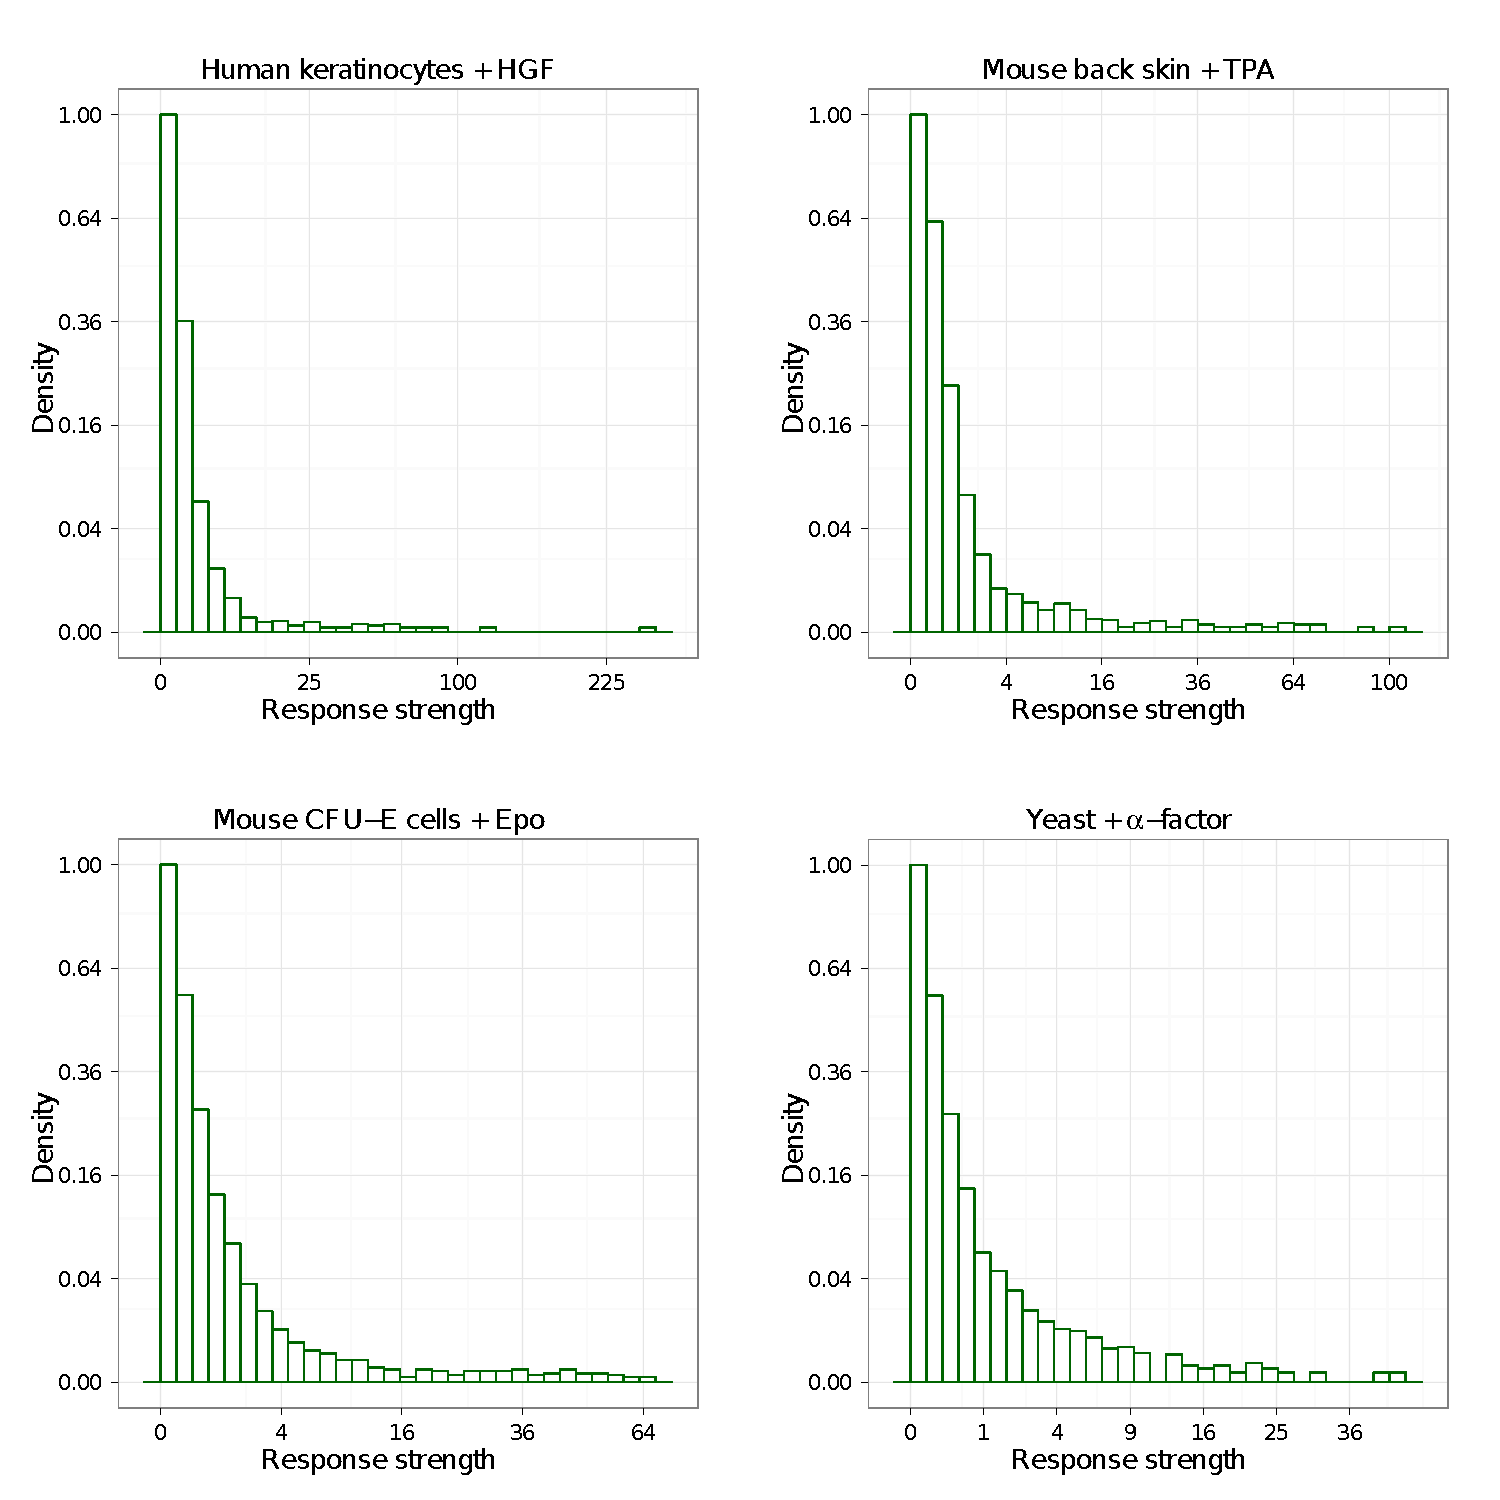
\includegraphics[width=\textwidth]{network/fig/response_all.pdf}
\end{center}
\caption[Heavy-tail distribution of gene response strength]{
{\bf Distribution of gene response strength in different
cell types under different stimulation.}
Gene response strengths are calculated as described in 
\ref{sec:response_strength}, the maximum of each distribution
is normalized to 1. Datasets used in this plot include 
primary human keratinocytes 
stimulated with hepatocyte growth factor (ArrayExpress database 
\texttt{http://www.ebi.ac.uk/arrayexpress/},
accession number E-TABM-440); CFU-E cells from mouse fetal livers stimulated
with Epo (GEO database \texttt{http://www.ncbi.nlm.nih.gov/geo/}, accession
number GSE26151); yeast cells synchronized with 
$\alpha$-factor to study the cell cycle
\\(\texttt{http://genome-www.stanford.edu/cellcycle/data/rawdata/combined.txt}).
}
\label{fig:response_strength}
\end{figure}

The response distributions do not fit well with any of the 
Gaussian, power-law, exponential, log-normal or Weibull distribution, with the closet one being power-law or log-normal
distribution up to a certain range (\ref{fig:response_fit}). 
Nevertheless, the response distributions from various 
biological systems do share the same shape between each 
other (\ref{fig:response_qqplot}). Taken together, gene
responses are indeed heavy-tail distributed, with few
genes strongly regulated and the majority only moderately
regulated, but they do not follow the power-law distribution,
which underlines again the necessity of assessing power-law
distribution on empirical data within a rigorous statistical
framework~\citep{Clauset2009}.

\begin{figure}[!ht]
\begin{center}
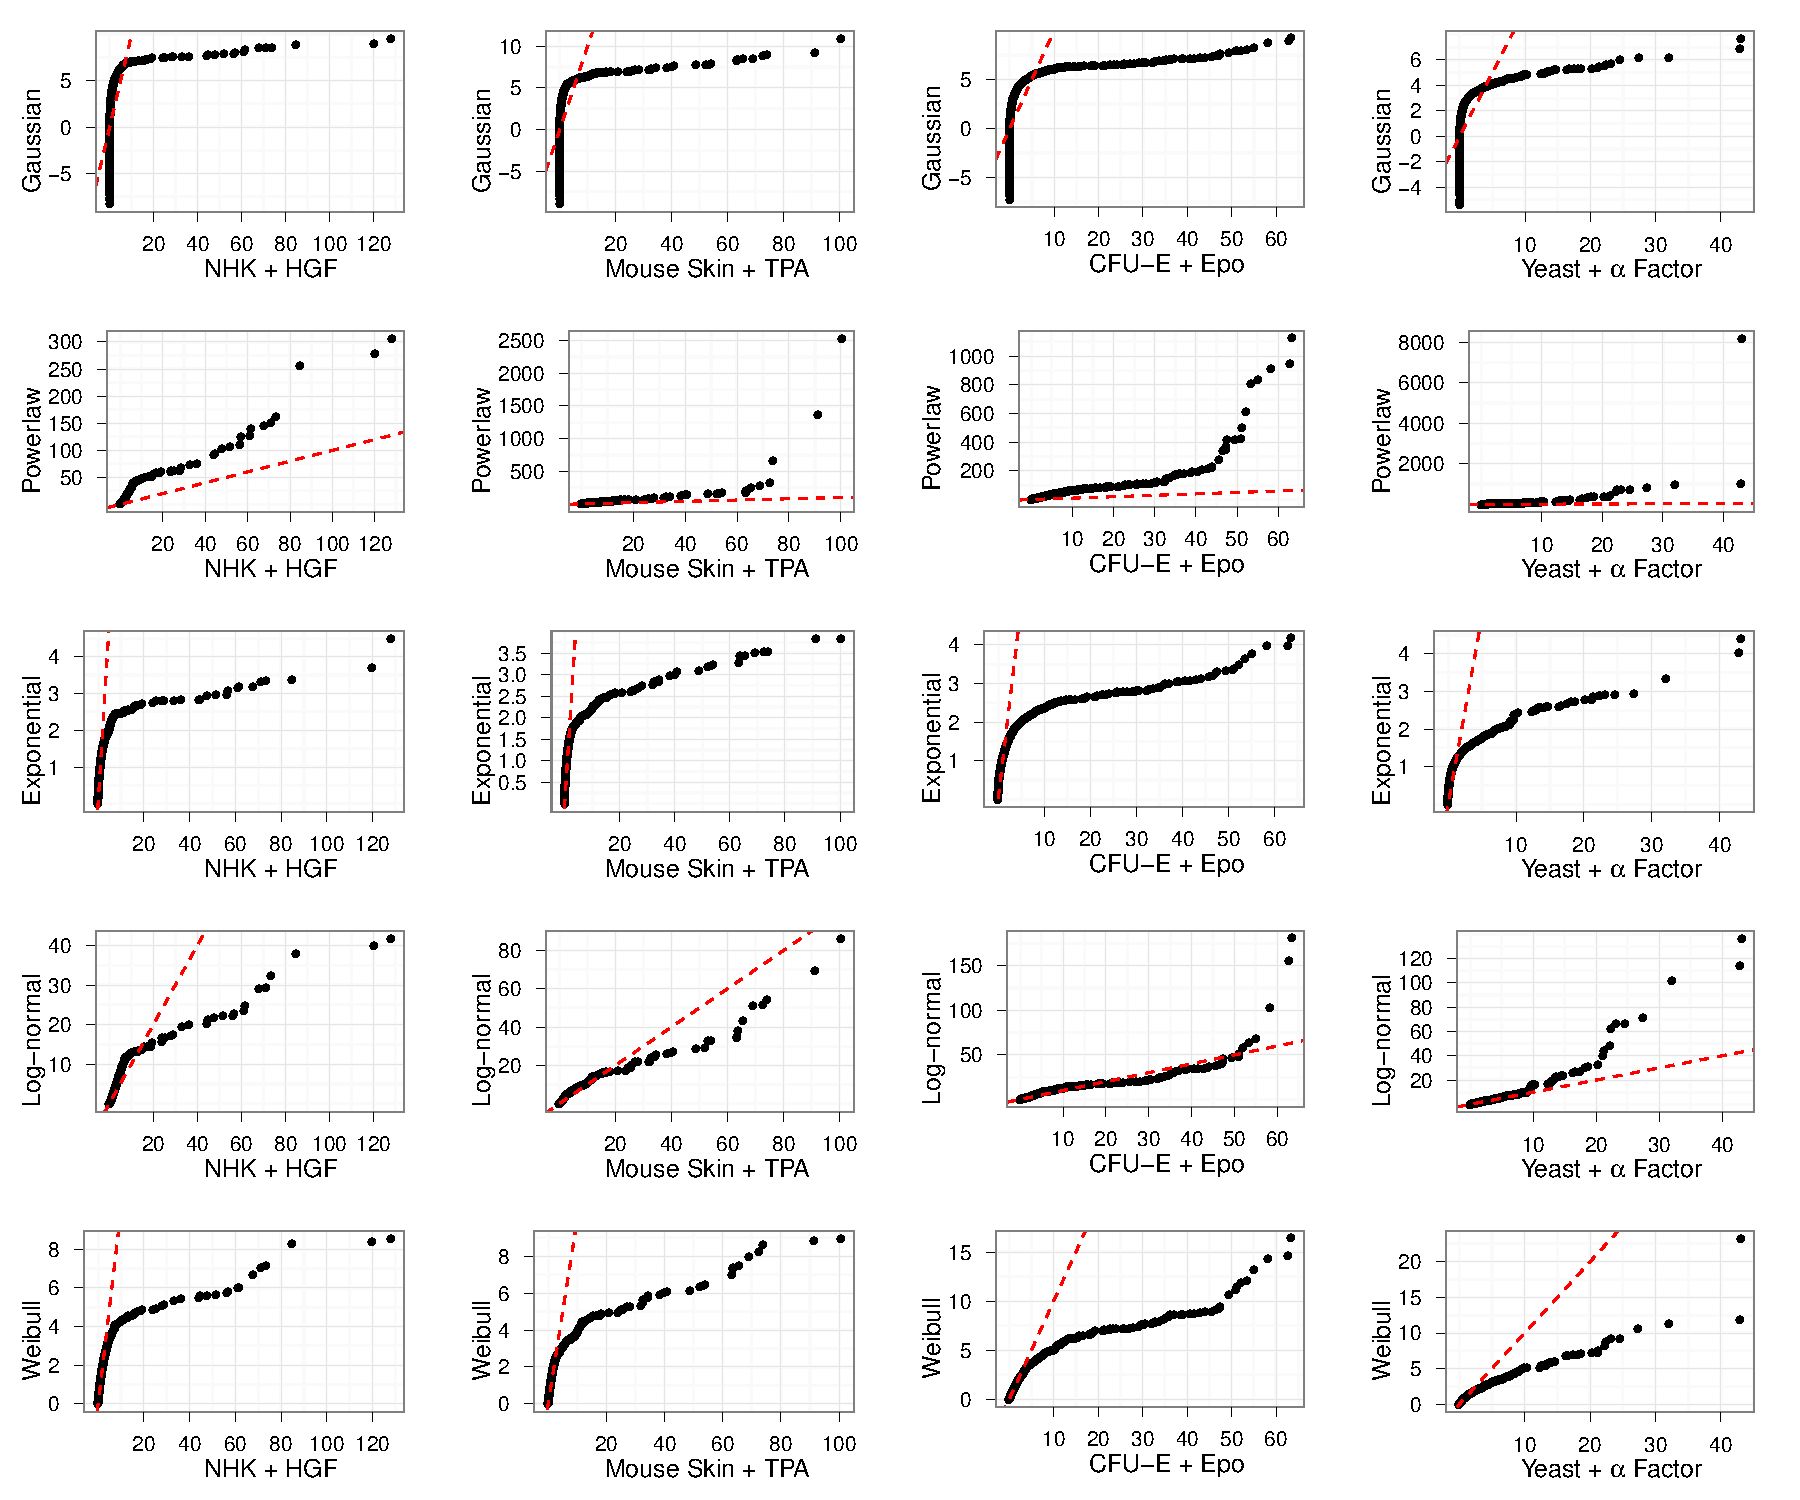
\includegraphics[width=\textwidth]{network/fig/response_fit.pdf}
\end{center}
\caption[Comparison of gene response distributions with
theoretical distributions]{
{\bf Comparison of gene response distributions with 
different theoretical distributions using the quantile-%
quantile plot.}
Biological datasets are the same as in 
\ref{fig:response_strength}, red dashed lines have a slope
of 1 and indicate identity, theoretical distributions 
include Gaussian, power-law, exponential, log-normal and
Weibull distribution~\citep{Clauset2009}.
}
\label{fig:response_fit}
\end{figure}

\begin{figure}[!ht]
\begin{center}
\includegraphics[width=\textwidth]{network/fig/response_qqplot.pdf}
\end{center}
\caption[Comparison of gene response distributions]{
{\bf Pairwise comparison of gene response distributions with 
each other using the quantile-%
quantile plot.} 
Biological datasets are the same as in 
\ref{fig:response_strength}, red dashed lines have a slope
of 1 and indicate identity, the maximal response strength
in each dataset is normalized to 1.
}
\label{fig:response_qqplot}
\end{figure}

One possible cause of the similar be behavior has been the similarity in underlying topology of the gene and protein regulatory network. 

\section{Gene response and connectivity}
Through the simulation of a thermodynamical gene network model, we observed that the response strength of a certain gene negatively correlates with its degree, which is also 
confirmed in various biological data.

\subsection{Synthetic \emph{in silico} networks}
We first describe the construction of \emph{in silico}
network models, both in terms of topology and dynamics.

\subsubsection{Topology}
\begin{itemize}
\item Random: an Erd\H{o}s-R\'enyi graph (\citealp{Erdos1959}) is generated with a probability
  $0.003$ to choose each of the possible edges.
\item Uniform: network with uniform in- and out-degree distributions $k_{in,out} \in 
  \{0,1,...,11\}$ is constructed 
  with the configuration model (\citealp{Newman2001}). 
  In short, a configuration network 
  is constructed in the following manner. Each node $i$ has a desired degree $k_i$, 
  so we imagine that each node has $k_i$ edge ``stubs'' attached to it. Edges are 
  then assigned by randomly choosing two stubs and drawing an edge between them.
\item Small-world: a small-world graph with 1000 nodes 
according to the 
Watts-Strogatz model~\citep{Watts1998} is generated, 
each node is connected
to 5 nearest neighbors in the ring topology and each edge
has a rewiring probability of 0.1. In the end, the 
undirected small-world graph is converted to a directed
graph by randomly assigning edge directions.
\item Scale-free: similar to the case of uniform networks,
except that Poisson in-degree (with $\lambda = 3$) and power-law 
  out-degree distributions ($P(k) = k^{-2.5}$) are assumed as the input
  to the configuration model.
\item Bow-tie: two growing network (GN) graphs 
  (\citealp{Krapivsky2001}) of equal size are first 
  constructed by adding nodes one at a time with an edge to one existing node, 
  which results in two directed trees. With redirection probability $0.1$ the edge
  connects the additional node with the successor node of the random selected target
  node instead of the target node itself. One of the trees is then reversed and 
  concatenated to the other one through the root nodes, such that the resulting
  graph is of the multiple-input multiple-output type.
\end{itemize}
All networks have 1000 nodes and are generated with the Python package NetworkX (\citealp{Hagberg2008}) 
version 1.4, they are further made sure to be connected.

\subsubsection{Dynamics}
We adapted a thermodynamical gene network model 
(\citealp{Marbach2010,Schilstra2002}),
which takes into account the combinatorial control of transcription factors. 
Precisely, the 
gene expression dynamics is defined by 
\begin{equation}
  \dot{x_i}(t) = m_i \cdot f_i(x_j(t)) - d_i \cdot x_i(t), 
\end{equation}
where $x_i(t)$ denotes the expression level of gene $i$ at time $t$, 
$m_i$ is the 
maximum transcription rate, $d_i$ the mRNA degradation rate. $f_i(\cdot)$
is the activation function of gene $i$, it depends on the expression level of 
all the input onto gene $i$ at time $t$, $x_j(t)$ and is the sum of relative 
activations for
different binding states. In general, for $N$ input genes, there are altogether
$2^N$ possible binding states and
\begin{equation}
  \displaystyle f_i(x_j) = \sum_{m=0}^{2^N-1} \alpha_m \theta_m,
\end{equation}
$m$ can be interpreted as an $N$-digit binary number (with padding $0$s) 
and represents one perticular binding state, with the $i$-th
digit indicating the binding state of the $i$-th input gene, namely $0$ for unbound
and $1$ for bound. $\alpha_m$ is the relative activation of state $m$,
$\theta_m$ is the joint probability of state $m$: 
\begin{equation}
  \theta_{m} = \prod_j \frac{x_j^{n_{ij}}}{k_{ij}^{n_{ij}}+x_j^{n_{ij}}}
    \cdot \prod_k \frac{k_k^{n_{ik}}}{k_{ik}^{n_{ik}}+x_k^{n_{ik}}}
\end{equation}
where the probability of a single transcription factor bound to the gene is 
modelled by a Hill function,
$n$ is the Hill coefficient and $k$ is the dissociation constant, at which the
saturation is half-maximal or the transcription factor is bound $50\%$ of the time.
$x_j$ are the bound transcription factors of $x_i$ and $x_k$ the unbound ones.

Time series are simulated by first finding the steady state, where the absolute
concentration change is smaller than $10^{-5} + 10^{-3} \cdot x_i$ for each gene
or the maximal time of $500$ is exceeded. Afterwards, the basal activation $\alpha_0$
is randomly perturbed and the gene expression dynamics is simulated for a total
time of $200$ with $10$ as the time interval and the
steady state as the initial condition.

\CC{} code of the model adapted from GeneNetWeaver (\citealp{Schaffter2011})
is available upon request.

\subsubsection{Rewiring}

\subsection{Topology determines dynamics}
We investigate the influence of network topology on the immediate, dynamic gene response in networks. 
Using biologically meaningful networks of \emph{E. Coli} and 
the budding yeast \emph{S. cerevisiae} generated 
\emph{in silico}, we show that topology has a significant influence on the dynamics, scaling with size. Hub genes are not responding, while weakly connected genes are 

Our results demonstrated that genes with a high level of change in expression are more likely to be peripheral nodes (low connectivity) in the network, whereas hubs (nodes with higher connectivity) and superhubs (nodes that link hubs) tend to have a lower level of change in expression. 
To analyze the biological roles of the modulated genes, we assessed the Gene Ontology (GO) of nodes and hubs. Our analysis identified different annotations of mole- cular functions based on the topological classifications.

\begin{figure}[!ht]
\begin{center}
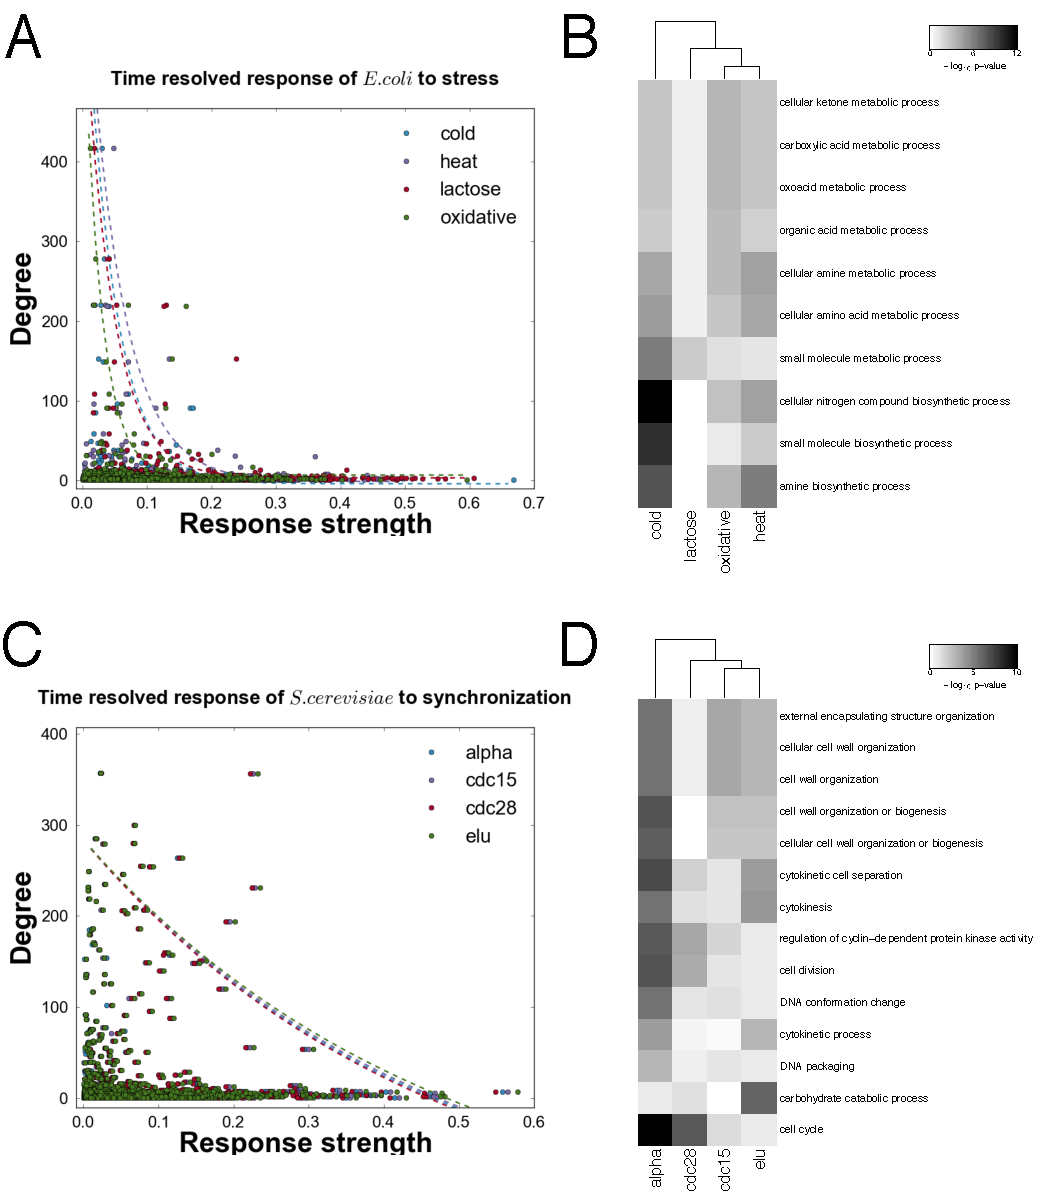
\includegraphics[width=\textwidth]{network/fig/ecoli_yeast_go.pdf}
\end{center}
\caption[GO term enrichment of strongly regulated genes]{
{\bf GO term enrichment of strongly regulated genes in the
\emph{E. coli} and yeast datasets.} 
}
\label{fig:response_qqplot}
\end{figure}

\section{Biological application}
We further went on to verify our hypothesis that strongly regulated peripheral 
genes are correlated with the phenotype by means of an \emph{in vitro}
mammalian cell system. Primary human keratinocytes extracted from the foreskin
migrate upon the treatment of hepatocyte growth factor (HGF), we measured
the gene expression profiles up to 8h after treatment of HGF (\citealp{Busch2008}) 
and identified
key genes with a large response strength according to MDS.

\subsection*{Invariant transcriptome response pattern}

%Cells coordinate their various functions as migration, proliferation or differentiation by regulation of their large gene interaction networks. To gain insight this gene network the usage of microarray analysis is nowadays state of the art. Time-dependent transcriptomic data are necessary to observe the dynamic response of cellular functions and decision. Fig.  (left panel) present the global gene response of different mammalian cells under diverse stimulation. The dynamic distributions of genes are ranked by the Multi-Dimensional Scaling (MDS) method (Figure 1, right panel). We quantify the relative dynamic response of all genes using a multi-dimensional scaling analysis (MDS). MDS embeds the high-dimensional distance matrix D of all pair-wise Euclidean distances between all gene expression kinetics into a low dimensional space, while conserving pair-wise distances \citealp{Strickert2009}.  Mapping the distance matrix $D$ onto a plane results in a cloud of points corresponding to the individual genes. Close or distant points represent genes with similar or dissimilar kinetics, respectively. We find the point cloud to be compact with few outliers, with the latter respresenting strongly responding genes having unique temporal expression profiles (Suppl. Fig. 7). 
Previous studies (\citep{Lu2007a,Mar2011}) have demonstrated a negative
correlation between the connectivity of a gene in the regulatory network
and its expression variance in the context of static disease models.
Here, we aim to address whether this negative correlation also exists 
between the network topology and its dynamic response.
In order to characterize the response strength over time of a certain gene, we
designed a metric based on multidimensional scaling (MDS). As a dimensionality 
reduction technique, MDS maps the high-dimensional gene expression profiles
to a low-dimensional space, while the relative pairwise distances are preserved
(\citealp{Taguchi2005,Tzeng2008}). Since genes with distinct kinetics have a
larger distance to the those with similar kinetics, and the dynamical behavior
is most likely a result of differential regulation, we created a metric to
describe the gene response strength based on its radial distance on the MDS
projection (Figure 1C right panel). In a real-world example where transcripts
are profiled in primary human keratinocytes under the stimulation of 
hepatocyte growth factor (HGF), we found the distribution of response
strengths has a long tail, indicating that 
only few genes are strongly induced by a certain stimulus, while the majority 
are barely regulated. Interestingly, this long-tail response strength
distribution is also observed in other cell types with various stimuli.
Among them are yeast cells that undergo cell cycles when synchronized by 
$\alpha$-factor, mouse skin cells stimulated with TPA and human Huh7.5 cells
under the stimulation of IFN-$\alpha$. It is known that the structures of
regulatory networks in various species are highly conserved 
(citation from Hauke), we thus hypothesize that this
universally invariant transcriptome response pattern results from the generic
topological features of the gene regulatory networks. Further questions 
arise, what distinguishes 
between the strongly and weakly responding genes? How is phenotype encoded 
in the gene network?

\subsection*{Topology is the determinant of dynamics in large networks}

To address the above questions, we applied biologically meaningful 
\emph{in silico} 
network models that are used to generate benchmark datasets for the DREAM 
(Dialogue for Reverse Engineering Assessments and Methods) challenge. The
model (\citealp{Marbach2010}) describes gene expression dynamics by the 
combinatorial regulation of upstream transcription factors. We constructed 
\emph{in silico} network models (Figure 2a) with a predefined topology from 
transcriptional regulatory networks in the \emph{E. coli} RegulonDB 
(\citealp{Gama-Castro2008}) 
and \emph{S. cerevisiae} (\citealp{Balaji2006}) or otherwise from a random,
uniform, scale-free or bow-tie network. Network dynamics was simulated after 
random 
multi-factorial perturbations from the steady state. Afterwards, the response 
strengths of individual genes are quantified by means of multidimensional 
scaling (Figure 2c). This workflow enables us to investigate how the dynamic
response pattern of a network relates to its topology. 

To first gain insight into the role that network topology plays, we compared
the different network responses after change of topology and change of kinetic 
parameters in an ensemble of \emph{E. coli} networks.
In the case of rewiring, we permutated the order of target nodes while keeping
the number of connections and kinetics parameters such as synthesis and 
degradation rates constant. Pearson correlation coefficients of the response
strengths before and after rewiring decrease slightly with the network size. 
In contrast, when we 
change the kinetic parameters without affecting the network topology (scheme, 
Figure 3A), the Pearson correlation coefficients remains at the same level and 
are in general higher than that before and after rewiring. The Kullback-Leibler
divergence, which measures the distance between two distributions, further 
confirms that the distance between the effect of rewiring and parameter change 
increases with the network size, indicating that network topology has a stronger 
impact on the response pattern, especially in large networks. 

\subsection*{Anti-correlation between connectivity and response}

To understand the functions of strong and moderate responders 
respectively, especially in a network point of view, we characterized
the relationship between the dynamic response of a node and its 
topological features with the help of an \emph{in silico} model of the
\emph{E. coli} network from RegulonDB. 
There is a weak but statistically significant
negative correlation between the degree of a gene and its response
strength. In other words, strong responders tend to have a low degree, 
whereas hub
genes with a high degree are hardly induced in general. We further characterized
the anti-correlation with a weighted exponential function, where the decay
constant $\lambda$ describes how strong this anti-correlation is.

With the help of the decay constant $\lambda$, we studied how the 
topology-response anti-correlation depends on the network structure.
While a hierarchically structured network, such as scale-free,
bow-tie networks, has a similar anti-correlation profile as the \emph{E. coli} 
network, random 
or uniform networks show a much higher variance in the anti-correlation between 
topology
and response. 

\subsection*{Strongly responding peripheral genes correlated with the phenotype}

The fact that strongly regulated genes always have a low degree and thus are
located at the periphery of the network poses the question whether these genes
mediate the computation of the whole network and then translate it into the 
phenotype. We therefore took the transcriptome data from the literature,
where time-resolved response of \emph{E. coli} (\citealp{Jozefczuk2010}) and 
\emph{S. cerevisiae} (\citealp{Spellman1998,Cho1998}) is 
measured under different stimuli. We found a similar anti-correlation between
network topology and response in the above datasets. Furthermore, we
carried out enrichment test of Gene Ontology (GO) terms in the significantly 
strong responders identified from MDS. For \emph{E. coli} cells in response
to different stress conditions, GO terms as metabolic processes, biosynthesis 
are over-represented in the strongly responding genes, which is in accordance
to the fact that cells have to adjust their growth rates under stress conditions.
On the other hand, for yeast cells in response to different synchronization
treatments, GO terms like cell wall organization, cytokinesis are more 
enriched than expected among strong responders, which is also in line with the
phenotype of cell cycles. Taken together, we found strongly induced genes, 
which are located at the periphery of gene regulatory networks, are nicely
correlated with the cellular phenotype.

\subsection*{Microarray datasets}

\section*{Figure Legends}

\paragraph*{Figure~1 }

Invariant transcriptome response patterns and the modelling approach. (A) 
Gene expression time series of primary human keratinocytes stimulated with 
hepatocyte growth factor (HGF). Histogram of the response strenth as determined by 
multidimensional scaling (MDS). (B) Histogram of the response strenth as determined by 
MDS for various cell types and stimuli. (C) Workflow to
investigate the relationship between topology and dynamics in a
thermodynamic model of cooperative gene regulation.
Time series are simulated after multi-factorial perturbations of the whole network.
MDS is applied to characterize dynamic response strengths
of individual genes.

\paragraph*{Figure~2 }

Effect of rewiring and parameter change on the network response 
pattern. (A) Schematic view of rewiring and the change of kinetic 
parameters, where black edges with a blunt head represent inhibiting
connections and red edges with an arrow head represent activating
connections, the values of kinetic parameters for each node are 
coded in gray scale. Dashed lines represent rewired edges. (B) Distribution 
of the correlation coefficients
before and after rewiring (change of parameters) in black (red) for 
different network sizes. (C) Kullback-Leibler divergence of the 
correlation coefficient distributions in B for different network
sizes.

\paragraph*{Figure~3 }

Correlation between the degree of a certain node in the network with its
response strength, which is defined by the radial distance in MDS.
Dashed lines are weighted exponential fits of the scatter plots from
1000 simulations with independent perturbations on the whole \emph{E. coli}
network from RegulonDB Version 6.2.

\paragraph*{Figure~4 }

Correlation between network dynamics and different topologies.
(A) Topology-respnose anti-correlation, as characterized by the decay constant 
$\lambda$, for different network structures. (B) Hierarchical clustering of 
different
network structures based on the Kullback-Leibler divergence between the $\lambda$
distributions.

\paragraph*{Figure~5 }

Strongly regulated peripheral genes are correlated with the phenotype.
(A) Topology-response anti-correlation of \emph{E. coli} in response 
to different stresses (extracted from \citealp{Jozefczuk2010}). (B) Topology-response
anti-correlation of \emph{S. cerevisiae} in response to different synchronizations
(extracted from \citealp{Spellman1998,Cho1998}). (C) Enrichment of GO terms
in the strongly induced peripheral genes of \emph{E. coli}. Shown are $p$-values
from Fisher's exact test in gray scale for different GO terms under different 
conditions. (D) Enrichment of GO
terms in the strongly induced peripheral genes of \emph{S. cerevisiae}. Shown 
are $p$-values
from Fisher's exact test in gray scale for different GO terms under different 
conditions.

\paragraph*{Figure~6 }



%\cleardoublepage{}
%
%\lhead[\fancyplain{}{}]{\fancyplain{}{Acknowledgments}}
%
%\rhead[\fancyplain{}{Acknowledgments}]{\fancyplain{}{}}
%
%
%
%\include{Appendix}

\cleardoublepage{}

\lhead[\fancyplain{}{}]{\fancyplain{}{\rightmark}}

\rhead[\fancyplain{}{\leftmark}]{\fancyplain{}{}}

\bibliographystyle{natbib}
\bibliography{diss,network/network}

\cleardoublepage{}

\lhead[\fancyplain{}{}]{\fancyplain{}{Nomenclature}}
\rhead[\fancyplain{}{Nomenclature}]{\fancyplain{}{}}

\printnomenclature{}

\chapter*{Acknowledgements}
\addcontentsline{toc}{chapter}{Acknowledgements}

%First off, I am grateful that Prof.~Ad Aertsen offered me this opportunity to 
%perform this work in the BrainWorks group. He not only oversees the whole 
%project, but discusses with me about the progress on a regular basis as well. 
%
%Dr.~Ralph Meier initiated the whole project and guided me through all the 
%essential literature concerning various hippocampal models of epilepsy.
%He also built a bridge between me and other experienced researchers in
%this field and allowed me to freely explore something new.
%
%I want to thank Dr.~Thomas Fucke, without whom the completion of this
%work would not have been possible. His stimulating ideas and constant
%encouragement are very much appreciated. Besides, Thomas' easy-going
%character makes him an ideal person to share an office with.
%
%There are numerous people, both experimentalists and theoreticians, 
%whom I have had discussion with and who have read
%and commented on the working copies of this thesis. I am also 
%fond of all the ``balcony breaks''.
%
%I am thankful to Huili, who is a good company and makes my life
%more colorful; to my parents for their unconditional support.

\newpage
\chapter*{Erkl\"arung}
\addcontentsline{toc}{chapter}{Declaration}
\begin{enumerate}
\item Ich erkl\"are hiermit, dass ich die vorliegende Arbeit ohne unzul\"assige Hilfe Dritter und ohne Benutzung anderer als der angegebenen Hilfsmittel angefertigt habe. Die aus anderen Quellen direkt 
oder indirekt \"ubernommenen Daten und Konzepte sind unter Angabe der Quellen gekennzeichnet. Insbesondere habe ich hierf\"ur 
nicht die entgeltliche Hilfe von Vermittlungs- beziehungsweise 
Beratungsdiensten (Promotionsberater oder anderer Personen) 
in Anspruch genommen. Niemand hat von mir unmittelbar oder 
mittelbar geldwerte Leistungen f\"ur Arbeiten erhalten, die im Zusammenhang mit dem Inhalt der vorgelegten Dissertation stehen.
\item Die Arbeit wurde bisher weder im In- noch im Ausland in gleicher 
oder \"ahnlicher Form einer anderen Pr\"ufungsbeh\"orde vorgelegt.
\item Die Bestimmungen der Promotionsordnung der Fakult\"at f\"ur Biologie der Universit\"at Freiburg sind mir bekannt, insbesondere 
wei\ss ich, dass ich vor Vollzug der Promotion zur F\"uhrung des 
Doktortitels nicht berechtigt bin.
\end{enumerate}
\vskip 3cm
Freiburg, den \ddmmyyyydate\today \hspace{6cm} Jie Bao

\end{document}
